% Use only LaTeX2e, calling the article.cls class and 12-point type.

\documentclass[12pt]{article}

% Users of the {thebibliography} environment or BibTeX should use the
% scicite.sty package, downloadable from *Science* at
% www.sciencemag.org/about/authors/prep/TeX_help/ .
% This package should properly format in-text
% reference calls and reference-list numbers.

\usepackage{scicite}

% Use times if you have the font installed; otherwise, comment out the
% following line.

\usepackage{times}

\usepackage{graphicx}

\usepackage{caption}
\usepackage{subcaption}

% The preamble here sets up a lot of new/revised commands and
% environments.  It's annoying, but please do *not* try to strip these
% out into a separate .sty file (which could lead to the loss of some
% information when we convert the file to other formats).  Instead, keep
% them in the preamble of your main LaTeX source file.


% The following parameters seem to provide a reasonable page setup.

\topmargin -1.0cm
\oddsidemargin 0.0cm
\textwidth 16cm 
\textheight 23cm
\footskip 1.0cm

%The next command sets up an environment for the abstract to your paper.

\newenvironment{sciabstract}{%
\begin{quote} \bf}
{\end{quote}}

% If your reference list includes text notes as well as references,
% include the following line; otherwise, comment it out.

%\renewcommand\refname{References and Notes}

% The following lines set up an environment for the last note in the
% reference list, which commonly includes acknowledgments of funding,
% help, etc.  It's intended for users of BibTeX or the {thebibliography}
% environment.  Users who are hand-coding their references at the end
% using a list environment such as {enumerate} can simply add another
% item at the end, and it will be numbered automatically.

\newcounter{lastnote}
\newenvironment{scilastnote}{%
  \setcounter{lastnote}{\value{enumiv}}%
  \addtocounter{lastnote}{+1}%
  \begin{list}%
  {\arabic{lastnote}.}
  {\setlength{\leftmargin}{.22in}}
  {\setlength{\labelsep}{.5em}}
}
{\end{list}}

\title{Lab Work 1} 

\author
{André Pedrosa [85098], Filipe Pires [85122], João Alegria [85048]\\
\\
Algorithmic Information Theory\\
\normalsize{Department of Electronics, Telecommunications and Informatics}\\
\normalsize{University of Aveiro}\\
} 

\date{\today{}}

%%%%%%%%%%%%%%%%% END OF PREAMBLE %%%%%%%%%%%%%%%%

\begin{document} 

% Double-space the manuscript.

\baselineskip18pt

% Make the title.

\maketitle 

% Place your abstract within the special {sciabstract} environment.

%\begin{sciabstract}
  
%\end{sciabstract}

% In setting up this template for *Science* papers, we've used both
% the \section* command and the \paragraph* command for topical
% divisions.  Which you use will of course depend on the type of paper
% you're writing.  Review Articles tend to have displayed headings, for
% which \section* is more appropriate; Research Articles, when they have
% formal topical divisions at all, tend to signal them with bold text
% that runs into the paragraph, for which \paragraph* is the right
% choice.  Either way, use the asterisk (*) modifier, as shown, to
% suppress numbering.

\section*{Introduction}

This report aims to describe the work developed for the first assignment
of the discipline of 'Algorithmic Information Theory', explaining all the 
steps and decisions taken by us, and presenting the results we considered 
most relevant.

The programs implemented in C++ have the purpose of collecting statistical
information about texts using Markov (finite-context) models, and of 
automatically producing texts that follows the models built.

Along with the description of the solution, we also discuss the effects
of the variation of the programs' parameters and attempt to compare 
different types of texts by the amount of information they hold on average.
\newpage

\section*{1. Information Model}

Our first goal was to be able to predict the next outcome of a text source.
To do this, we needed to take in consideration the dependencies between 
the characters of a text.
The use of Markov models for the extraction of the statistical properties of a
text was due to its value as an approach to represent these data dependencies.

The specific type of model that most interests us is called discrete time
Markov chain or finite-context model.
This model assigns a probability estimate to the symbols of the alphabet, 
according to a conditioning context computed over a finite and fixed number
of past outcomes. 
More about this is explained in the description of this work assignment 
\cite{trab1}, containing the mathematical equations that served as the basis 
for our implementation.

\subsection*{1.1. Collecting Data}

We decided to organize the program by several files, each with a different
purpose, for good readability and to allow future modifications without the 
need of much refactoring - so we adopted a modular architecture strategy.

The file \texttt{fcm.cpp} serves as the base code for the command to be executed in order to 
generate a finite-context model, given one or several information source(s).
By executing this command, the program is started and begins to
call a set of functions that return an instance of our 
implementation of the Markov's model trained from the information source(s), 
and calculate the text entropy, as estimated by this instance.
The \texttt{fcm} command has the following format:

\begin{quote}
\begin{verbatim}
$ ./fcm [-h] k alpha trainFile [trainFile ...]
\end{verbatim}
\end{quote}

Here, \texttt{-h} is the option that presents the manual for the command usage.
Argument \texttt{k} is the value given for the size of the context.
This context corresponds to a string with \texttt{k} characters, it is based on
the several contexts produced and on the single characters that follow each one
of them that the model is able to calculate the text's entropy.
\texttt{alpha} stands for the value of the 'smoothing' parameter for estimating
the probabilities of events. 
These events correspond to the occurrences of a character after a given context.
And \texttt{trainFile} is, as the name indicates, the name of the file(s) that
contain the text to be processed by the model.

First, the command executed is pre-processed and its arguments are collected
and validated by the function {\it parseArguments()\/}, implemented in 
\texttt{argsParsing.cpp} and defined in \texttt{argsParsing.h}.
The use of a header file is to establish an interface for the possibility of
creating different implementations of the parsing functions.
This is also visible in the implementation of the Model class in files 
\texttt{model.cpp} and \texttt{model.h}.

Once the arguments are validated, the program attempts to open the file(s) for reading
through function {\it checkAccess()\/} and, in case of success, reads and parses
its content.
The program supports any file format as long as its content is plaintext.
<<<<<<< HEAD
=======

>>>>>>> ce72ddbaa94171a49b87c19aa1ba6ee5804ef7aa
Below we present the actual implementation in C++ of the function responsible 
for parsing the information source file.

Variable \texttt{abc} contains the alphabet of the input file, updated everytime
a new character is found.
The function {\it parseFile()\/} creates a copy of this alphabet and a new
alphabet that will contain the new found characters (if any).
It then iterates over the file's content letter by letter, inserts each on both
alphabets (if not already in them), updates the number of occurrences of each 
letter after the corresponding context and updates total number of contexts in 
each iteration.
Once the end of file (EOF) is reached, the function calls 
{\it calcProbabilitiesAndEntropy()\/}.

\begingroup
\addtolength\leftmargini{-0.4in}
\addtolength\baselineskip{-0.05in}
\begin{quote}
\begin{verbatim}
void Model::parseFile(list<fstream*> &input) {
  [...]
  for (auto reader : input) {
      while (reader->get(letter)) {
          abc.insert(letter);
          if (context.length() >= ctxLen) {
              statsTable[context].nextCharStats[letter].count++;
              statsTable[context].stats.count++;
              totalContextsCount++;
              context = context.substr(1);
          }
          context += letter;
      }
  }
  calcProbabilitiesAndEntropy();
}
\end{verbatim}
\end{quote}
\endgroup

This solutions makes our model prepared to accept more than one information
source (i.e. several input files).
Although this was not a requirement, we knew this would make the program more
robust and scalable.

\newpage

\subsection*{1.2. Training the Model and Returning Text Entropy}

Finally, as the file is parsed and the alphabet is built, \texttt{fcm} then 
builds the information table containing the statistics of the input text and
calculates the estimated value for the entropy through the function
{\it calcProbabilitiesAndEntropy()\/}. 
To build the information table, we followed a dictionary approach where we have 
a first level dictionary with the context string as key and a structure 
(ConstextStatistics) as value.
This structure contains another structure (Statistics) with statistics 
(number of occurrences and probability) about that context and a dictionary.
This second layer dictionary has, as key, a letter of the alphabet and, as 
value, the statistics structure mentioned above, but this time the data is 
relative to occurrences of a letter after a context.

As all contexts' and letters' number of occurrences are calculated on the
method {\it parseFile()}, on {\it calcProbabilitiesAndEntropy()} we
calculate their probabilities. 
The context's probability is given by its number of occurrences divided 
by the sum of occurrences of all contexts, in other words, the total number 
of contexts in all training data.
A letter's conditional probability is obtained by dividing the number of 
occurrences after a given context by the number of occurrences of that context.

To calculate these probabilities we iterate over the two layer dictionary.
On the first layer of the dictionary we calculate probabilities related to
contexts (\(P(c)\)) and while iterating over the second layer we calculate
the context entropy (\(H_c\)). 
For a given context, not all letters of the alphabet appear after it.
This brought us trouble for the second assignment's task so, to fix it,
we make a copy of the alphabet, remove the ones that appeared, set their 
count to 0 and only then calculate the conditional probability.

Calculating all this allows us to avoid having to iterate over the entire 
table more than once in order to calculate the model's entropy or the 
conditional probabilities for each letter after each context.

\newpage

The mathematical equations required for the calculation of the entropy are 
available in the document that describes the assignment. 
% The actual work was to implement these formulas and apply them.

The function {\it calcProbabilitiesAndEntropy()\/} is presented next for further
analysis.

\begingroup
\addtolength\leftmargini{-0.4in}
\addtolength\baselineskip{-0.05in}
\begin{quote}
\begin{verbatim}
  void Model::calcProbabilitiesAndEntropy() {
    [...]
    for (auto &it: statsTable) {
        contextStats = &it.second;
        contextCount = contextStats->stats.count;
        contextStats->stats.probability = 
          (double)contextCount / totalContextsCount;
        set<char> abcCopy(abc);
        for (auto &it2: contextStats->nextCharStats) {
            letter = it2.first;
            stats = &it2.second;
            charCount = stats->count;
            conditionalProb = (charCount + alpha)
                / (contextCount + alpha * abc.size());
            stats->probability = conditionalProb;
            Hc += conditionalProb * log2(conditionalProb);
            abcCopy.erase(letter);
        }
        for (char l: abcCopy) {
            conditionalProb = alpha
                / (contextCount + (alpha * abc.size()));
            contextStats->nextCharStats[l] = 
                {0, conditionalProb};
            if (conditionalProb > 0) {
                Hc += conditionalProb * log2(conditionalProb);
            }
        }
        Hc = -Hc; 
        entropy += contextStats->stats.probability * Hc;
        Hc = 0.0;
    }
  }
\end{verbatim}
\end{quote}
\endgroup
\newpage

\section*{2. Text Generator}

The second part of the assignment was to developed a program for automatic
text generation that follows the statistical model learned beforehand using 
a training text.
To do this, we use \texttt{model.cpp} as a starting point and developed 
\texttt{generator.cpp}. 
This program, similarly to \texttt{fcm}, works as a command when executed.
\texttt{generator} starts by passing the information source(s) to the 
\texttt{model.cpp}, that internally will construct the Markov's model 
following the same dataflow as \texttt{fcm} when processing the file. 
Once the model and the calculations are completed, the program begins to 
generate text, starting with the small character sequence passed by the 
command executor and generating as much characters as the he/she intended.

The \texttt{generator} command has the following format: 

\begin{quote}
\begin{verbatim}
$ ./generator [-h] k alpha beginSequence numChars \\
outputFile trainFile [trainFile ...]
\end{verbatim}
\end{quote}

Once again we have the \texttt{-h} option that presents the manual for the 
command usage.
Arguments \texttt{k} and \texttt{alpha} are the same as the ones on the 
command \texttt{fcm}.
The \texttt{beginSequence} argument asks the user to give a word or character
sequence for the program to start off from; this is a need instrinsic to the
way the solution works and must be the same length as the context lenght.
The \texttt{numChars} argument tells the program how many characters are to be outputed.
The \texttt{outputFile} is where the generated text will be written to.
Finally the \texttt{trainFile} is, as the name suggests, the name of the file(s) to be
processed by the model and used as training.

Bellow we present a small portion of a text generated by our solution 
after training it with the information source file \texttt{alice\_oz.txt}
and passing \texttt{...} as the {\it beginSequence\/}.

\newpage
\section*{3. Results}

In this chapter we discuss the results achieved from the final version of 
both tasks solutions. 
During development, we used randomly generated texts to test our code.
However, for the analysis described here, we used two text files
containing {\it The Bible\/} in plaintext, one written in English 
(\texttt{bible\_en\_v1.txt}) and the other in Portuguese 
(\texttt{bible\_pt.txt}).
The reason we chose the same text source translated in different languages
was to evaluate the entropy of each language and compare them in terms of 
average quantity of information per character of the alphabet.
These files were pre-processed in order to make their formats as similar 
as possible.

\subsection*{3.1. Parameter Variation}

We defined a few assumptions after considering the problem of determining
the entropy of an information model and aimed to test them out once the 
program was completed.
In this section we explain these hipothesis and analyse their truthfulness
with the aid of a graphic plotting the evolution of the text entropy with
parameters k and $\alpha$ as variables.
It is important to state that our assumptions are based on the interpretation
of the mathematical formulas around the model implemented and that they 
are supposed to apply to texts of any size.

Taking a closer look at the formula for the overal entropy of the model 
(equation 1), we can gather that as the context probability 
decreases so does the value of the entropy.
But what exactly affects the probability of a context? 
Assuming we start from an equal probability of occurring any of the existing
contexts, the more contexts there are, the less probability there is of 
occurring a specific one.
Also, for a given text source, the longer the context is (substring of fixed 
size from the text source), the more possible combinations of letters there 
are and, consequently, the more unique contexts appear on the given text.
Taking this in consideration, we are able to establish that increasing the 
context size results in an increase of the total number of different contexts
and, consequently, in a decrease of the probability of occurring each context
and finally leading to a decrease in the final value for the model's entropy
(see equation 2).

\begin{equation}
  H = \sum\limits_{c} P(c) Hc
\end{equation}
\begin{equation}
  >size(c) \Rightarrow <P(c) \Rightarrow <H
\end{equation}

Our second hypothesis regarded the 'smoothing' parameter $\alpha$.
The idea behind this parameter is to tackle the issue of constructing the
model and assigning zero probability to unseen events.
By adding $\alpha$, the character probabilities is uniformized and they 
never actually reach zero.
As we studied the effects of the variable on the formula of conditional 
probabilities (see equation 3), we came to the conclusion that the larger
its value, the bigger will be the model's entropy.

\begin{equation}
  P(e|c) \approx \frac{N(e|c) + \alpha}{\sum\limits_{s\in\Sigma}N(s|c) + \alpha|\Sigma|}
\end{equation}

This was harder to reach as, at first sight, the effect of $\alpha$ is only 
relevant in a binary way, i.e. it affects the result if it is bigger than 
zero (the same way, no matter its value), it does not if not.
However, by analysing the situation more carefully, we understood that,
assuming that $\alpha$ is bigger than zero, the larger its value, the smaller
is the bottom parcel of equation 3 and, consequently the larger the 
conditional probability is.
From that point on, one can understand that the larger the $\alpha$, the larger
will be the entropy.\\

We developed a script in \texttt{Matlab} that runs \texttt{fcm.cpp} a
defined number of times for the same source of information varying the 
two studied parameters in several combinations.
This script collects the entropy values for each combination and then plots
them in a line graph.
Our next step was to run the script for the file 
\texttt{bible\_en\_processed.txt}, varying k between 1 and 6, and $\alpha$ 
between 0 and 1.
Figure \ref{graph} shows the resulting plot.

\begin{figure}[h!]
  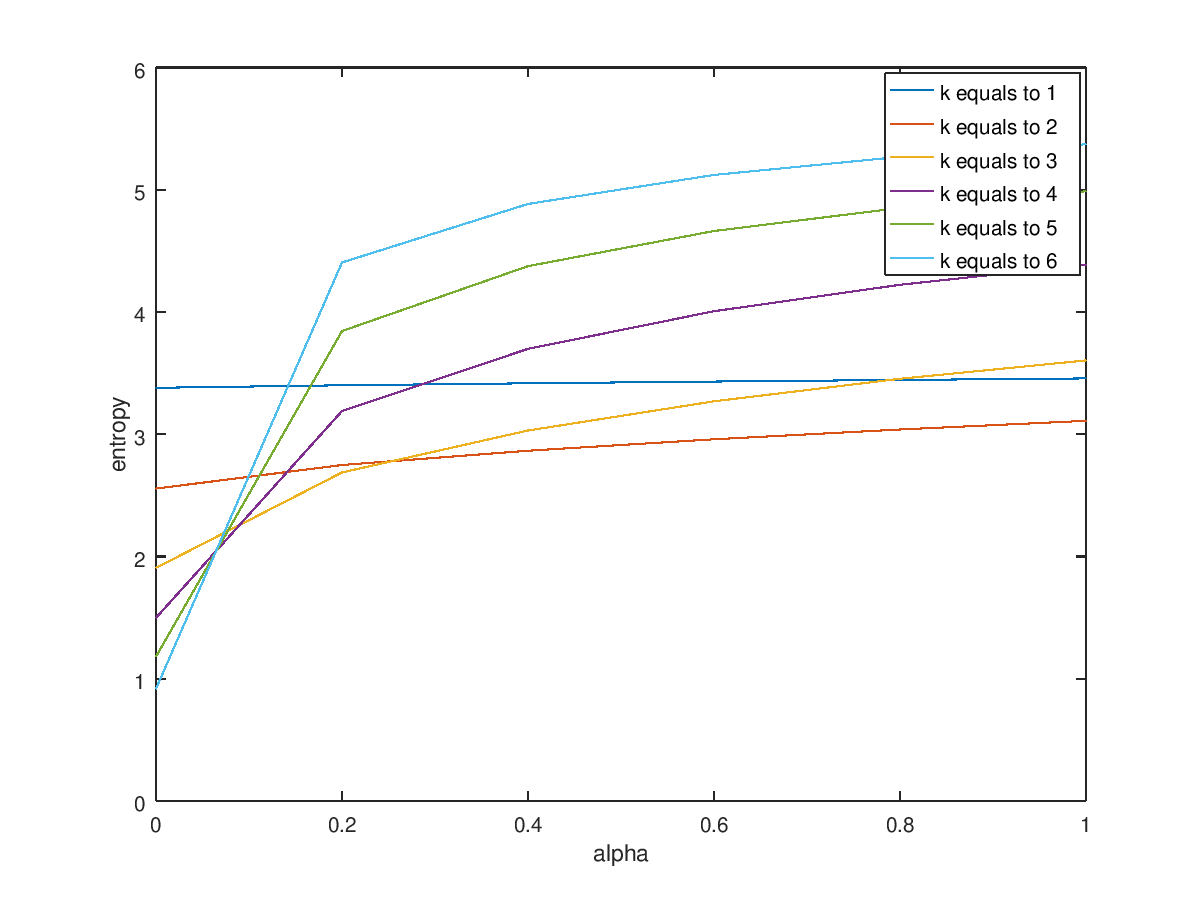
\includegraphics[width=\linewidth]{graph.png}
  \caption{Entropy evolution in relation to alpha to different context sizes}
  \label{graph}
\end{figure}

As one can verify by looking at Figure \ref{graph}, the value for the text
entropy has a sort of logarithmic growth as the $\alpha$ increases; this is 
visible for any k, although the growth rate is reduced as k gets smaller.
This observation confirms our second hypothesis and helps us understand with
greater detail the influence of $\alpha$ on our information model.

The entropy's evolution according to the k values is a little bit trikier.
Our hypothesis that stated that the larger the k value is the smaller will
the entropy be is confirmed when $\alpha$ values are close to zero.
As there is no normalization process (achieved by larger $\alpha$ values),
the entropy evolves the way we predicted it to.
What $\alpha$ does here is reducing the effect of the context's size on the 
final value of the model's entropy.

Another observation we made when studying parameters variations was related
to the size of the texts used as information sources.
..............................

\subsection*{3.2. Text Comparison}

\begin{figure}
  \centering
  \begin{minipage}{.5\textwidth}
    \centering
    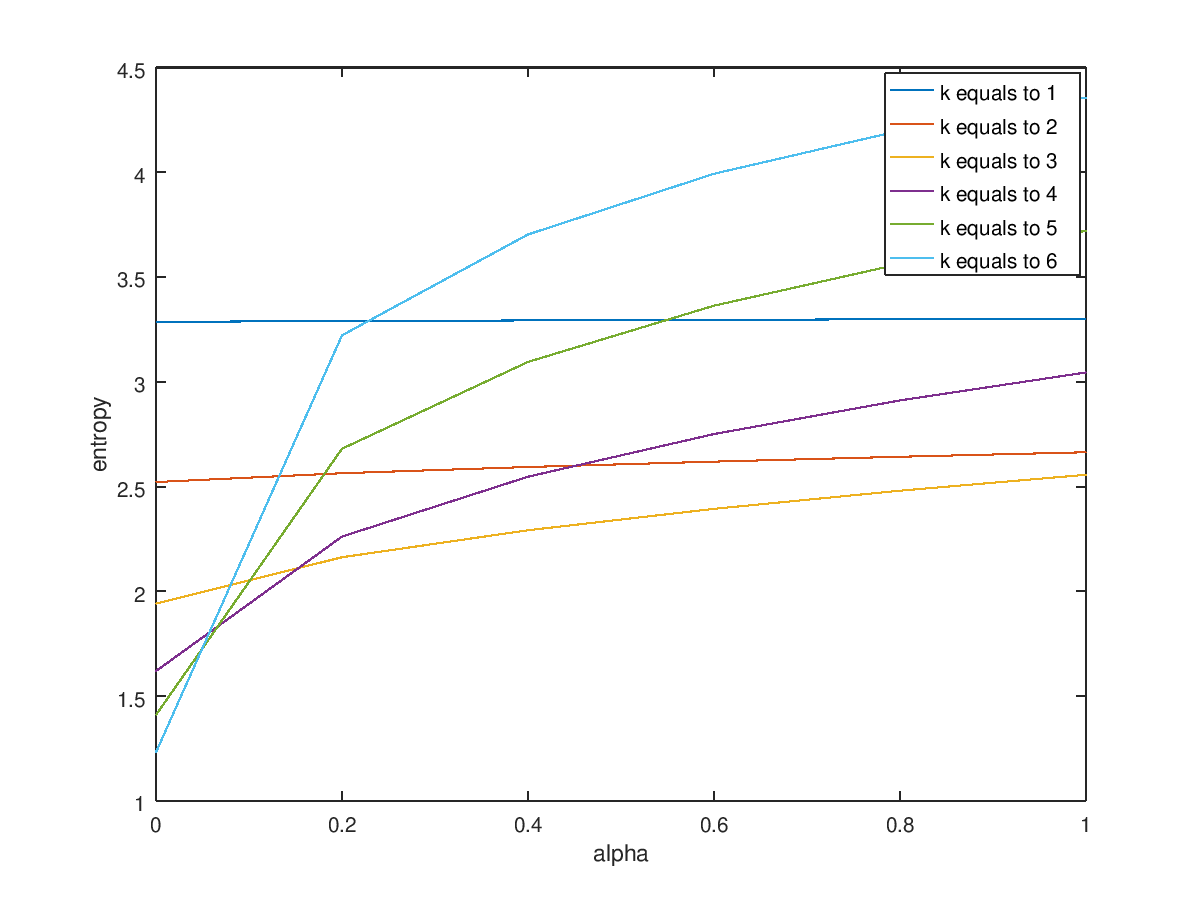
\includegraphics[width=\linewidth]{bible_v1.png}
    \captionof{figure}{English Bible Entropy}
  \end{minipage}%
  \begin{minipage}{.5\textwidth}
    \centering
    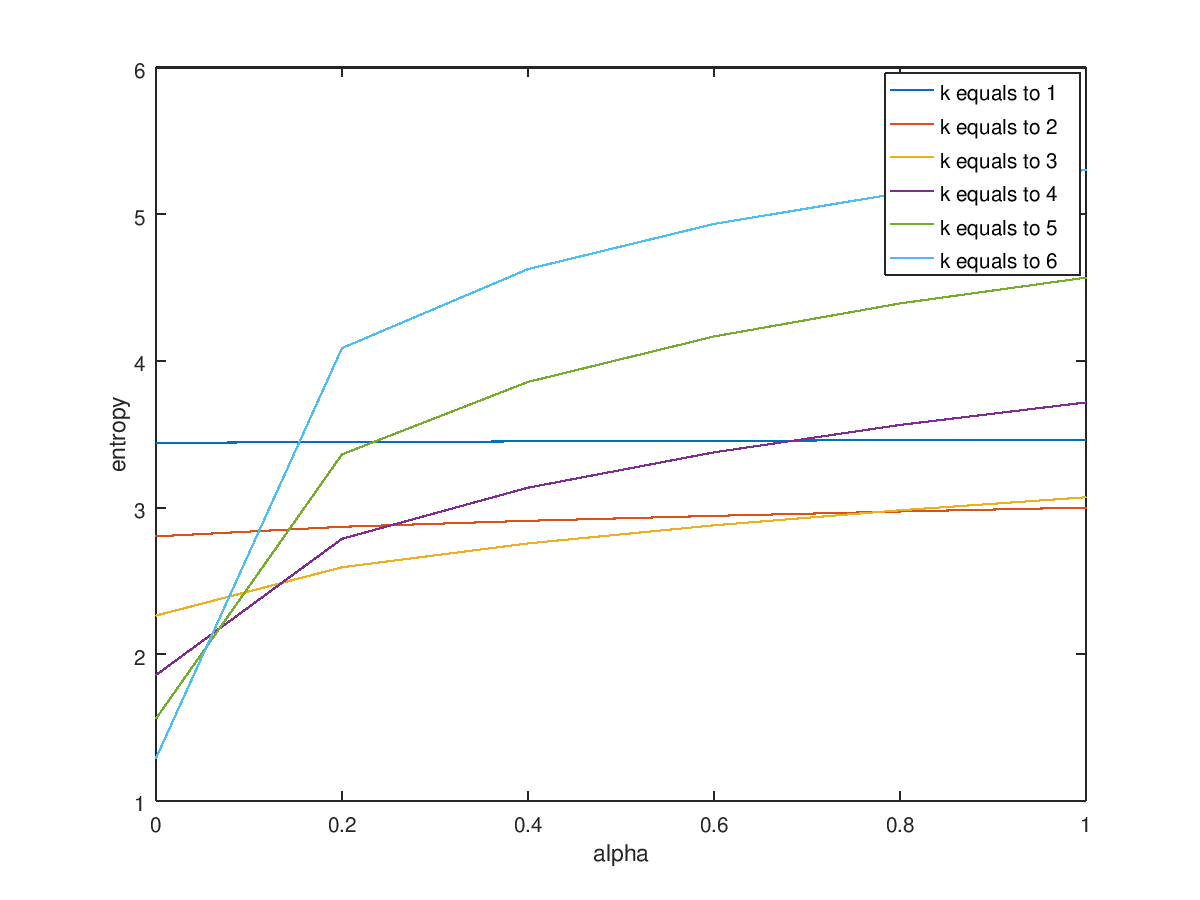
\includegraphics[width=\linewidth]{bible_pt.png}
    \captionof{figure}{Portuguese Bible Entropy}
  \end{minipage}
  \end{figure}

As a curiosity we thought on calculating the entropy to different languages to assert if languages differ in entropy and if so, what causes those variations. For this we used again the \texttt{bible\_en\_processed.txt} in addition to the \texttt{bible\_pt\_processed.txt} to compare the English language to the Portuguese language. We purposefully used the same document in different languages to maintain the message itself, so this way we can compare the languages entropies to a given message, normalizing the process.
The results can be observed in \texttt{Figure 2} and \texttt{Figure 3}, and as expected the entropy behavior is the same as already explained in section \texttt{Parameter Variation}. Taking a closer look, observing the entropy values to alpha equal to 0, we see a small difference between the two, where the values are:

\subsection*{3.3. Generator's Response to Parameter Variations}

Lorem ipsum ...

\section*{Conclusions}

Lorem ipsum ...

\begin{thebibliography}{9}
  \bibliographystyle{Science}

  \bibitem{trab1}
    Armando,
    \textit{AIT: Lab Work no.1},
    University of Aveiro,
    2019/20.
  
\end{thebibliography}

\clearpage

\end{document}




















